\documentclass[11pt]{article}
\usepackage[a4paper,margin=1.8cm]{geometry}
\usepackage{tikz}
\usepackage{amsmath}
\setcounter{MaxMatrixCols}{10}
\usepackage{amssymb}
\usepackage{xcolor}
\pagestyle{empty}

\begin{document}
\section*{$S=\{0,1,3,4\}$, $m=4$, $t=6$}
\begin{center}
$\mathbf{FAILURE}$
\end{center}
$\left\lfloor t/2\right\rfloor=3$
\quad\quad
$J=\{1,2,3\}$
\quad\quad
$N=0$
\quad\quad
$\operatorname{rank}(Y^{+})=0$

\begin{center}
\smallskip Complete graph on $V$, with vertices in $S$ and edges in $E(S)$ highlighted in red. $|E(S)|=6$

\begin{minipage}[t]{0.31\textwidth}
\centering
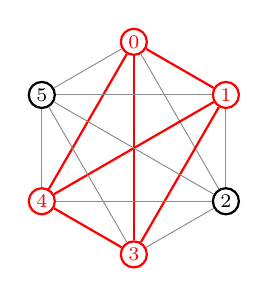
\begin{tikzpicture}[
  thick,
  baseline=(current bounding box.north),
  vertex/.style={circle,draw,inner sep=1.2pt,font=\scriptsize},
  svertex/.style={circle,draw=red,text=red,inner sep=1.2pt,font=\scriptsize}
]
  \node[svertex] (v0) at (0.000,1.350) {0};
  \node[svertex] (v1) at (1.169,0.675) {1};
  \node[vertex] (v2) at (1.169,-0.675) {2};
  \node[svertex] (v3) at (0.000,-1.350) {3};
  \node[svertex] (v4) at (-1.169,-0.675) {4};
  \node[vertex] (v5) at (-1.169,0.675) {5};
  \draw[red] (v0) -- (v1);
  \draw[black!45,line width=0.35pt] (v0) -- (v2);
  \draw[red] (v0) -- (v3);
  \draw[red] (v0) -- (v4);
  \draw[black!45,line width=0.35pt] (v0) -- (v5);
  \draw[black!45,line width=0.35pt] (v1) -- (v2);
  \draw[red] (v1) -- (v3);
  \draw[red] (v1) -- (v4);
  \draw[black!45,line width=0.35pt] (v1) -- (v5);
  \draw[black!45,line width=0.35pt] (v2) -- (v3);
  \draw[black!45,line width=0.35pt] (v2) -- (v4);
  \draw[black!45,line width=0.35pt] (v2) -- (v5);
  \draw[red] (v3) -- (v4);
  \draw[black!45,line width=0.35pt] (v3) -- (v5);
  \draw[black!45,line width=0.35pt] (v4) -- (v5);
\end{tikzpicture}
\end{minipage}
\par\smallskip Jumps in $E(S)$: $J=\{1,2,3\}$
\par $b_{01} + b_{34} + b_{04} + b_{13} + b_{03} + b_{14} \le d_m(|S|)=d_{4}(4)=5$
\par $2 y_{1} + 2 y_{2} + 2 y_{3} \le 5$
\end{center}

Each drawing below is a circulant graph $G_{L}$ for a non-empty $L\subseteq J$ with edges $E(L)=\{\{i,j\}\mid i,j\in V,\ \min((i-j)\bmod t,\,(j-i)\bmod t)\in L\}$.
For each graph, we show $|E(L)\cap E(S)|$ and put $\textcolor{green!60!black}{\checkmark}$ iff $|E(L)\cap E(S)|=d_m(|S|)$; otherwise $\textcolor{red}{\boldsymbol{\times}}$.
When a checked graph is minimal under single-jump deletion, we append $\textbf{MIN}$ right after the checkmark.
All non-empty jump sets are shown.

\noindent
\begin{minipage}[t]{0.31\textwidth}
\centering
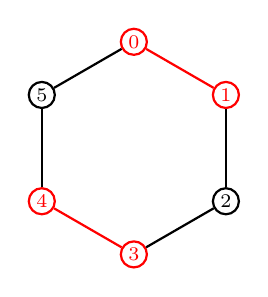
\begin{tikzpicture}[
  thick,  vertex/.style={circle,draw,inner sep=1.2pt,font=\scriptsize},  svertex/.style={circle,draw=red,text=red,inner sep=1.2pt,font=\scriptsize},  baseline=(current bounding box.north)
]
  \node[svertex] (v0) at (0.000,1.350) {0};
  \node[svertex] (v1) at (1.169,0.675) {1};
  \node[vertex] (v2) at (1.169,-0.675) {2};
  \node[svertex] (v3) at (0.000,-1.350) {3};
  \node[svertex] (v4) at (-1.169,-0.675) {4};
  \node[vertex] (v5) at (-1.169,0.675) {5};
  \draw[red] (v0) -- (v1);
  \draw (v0) -- (v5);
  \draw (v1) -- (v2);
  \draw (v2) -- (v3);
  \draw[red] (v3) -- (v4);
  \draw (v4) -- (v5);
\end{tikzpicture}
\par\smallskip Graph 1
\par $L=\{\textcolor{red}{1}\}$
\par $y=\left(\textcolor{red}{1},\textcolor{red}{0},\textcolor{red}{0}\right)$
\par $|E(L)\cap E(S)|=2\;\;\textcolor{red}{\boldsymbol{\times}}$
\end{minipage}\hfill\begin{minipage}[t]{0.31\textwidth}
\centering
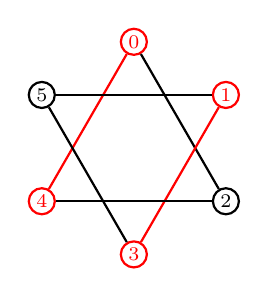
\begin{tikzpicture}[
  thick,  vertex/.style={circle,draw,inner sep=1.2pt,font=\scriptsize},  svertex/.style={circle,draw=red,text=red,inner sep=1.2pt,font=\scriptsize},  baseline=(current bounding box.north)
]
  \node[svertex] (v0) at (0.000,1.350) {0};
  \node[svertex] (v1) at (1.169,0.675) {1};
  \node[vertex] (v2) at (1.169,-0.675) {2};
  \node[svertex] (v3) at (0.000,-1.350) {3};
  \node[svertex] (v4) at (-1.169,-0.675) {4};
  \node[vertex] (v5) at (-1.169,0.675) {5};
  \draw (v0) -- (v2);
  \draw[red] (v0) -- (v4);
  \draw[red] (v1) -- (v3);
  \draw (v1) -- (v5);
  \draw (v2) -- (v4);
  \draw (v3) -- (v5);
\end{tikzpicture}
\par\smallskip Graph 2
\par $L=\{\textcolor{red}{2}\}$
\par $y=\left(\textcolor{red}{0},\textcolor{red}{1},\textcolor{red}{0}\right)$
\par $|E(L)\cap E(S)|=2\;\;\textcolor{red}{\boldsymbol{\times}}$
\end{minipage}\hfill\begin{minipage}[t]{0.31\textwidth}
\centering
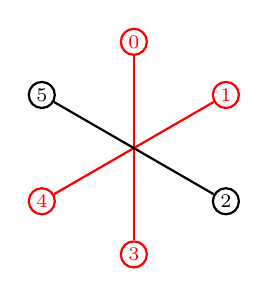
\begin{tikzpicture}[
  thick,  vertex/.style={circle,draw,inner sep=1.2pt,font=\scriptsize},  svertex/.style={circle,draw=red,text=red,inner sep=1.2pt,font=\scriptsize},  baseline=(current bounding box.north)
]
  \node[svertex] (v0) at (0.000,1.350) {0};
  \node[svertex] (v1) at (1.169,0.675) {1};
  \node[vertex] (v2) at (1.169,-0.675) {2};
  \node[svertex] (v3) at (0.000,-1.350) {3};
  \node[svertex] (v4) at (-1.169,-0.675) {4};
  \node[vertex] (v5) at (-1.169,0.675) {5};
  \draw[red] (v0) -- (v3);
  \draw[red] (v1) -- (v4);
  \draw (v2) -- (v5);
\end{tikzpicture}
\par\smallskip Graph 3
\par $L=\{\textcolor{red}{3}\}$
\par $y=\left(\textcolor{red}{0},\textcolor{red}{0},\textcolor{red}{1}\right)$
\par $|E(L)\cap E(S)|=2\;\;\textcolor{red}{\boldsymbol{\times}}$
\end{minipage}
\par\medskip
\noindent
\begin{minipage}[t]{0.31\textwidth}
\centering
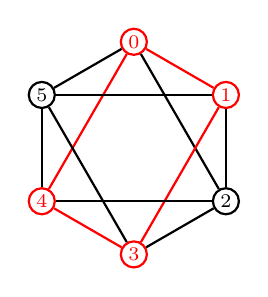
\begin{tikzpicture}[
  thick,  vertex/.style={circle,draw,inner sep=1.2pt,font=\scriptsize},  svertex/.style={circle,draw=red,text=red,inner sep=1.2pt,font=\scriptsize},  baseline=(current bounding box.north)
]
  \node[svertex] (v0) at (0.000,1.350) {0};
  \node[svertex] (v1) at (1.169,0.675) {1};
  \node[vertex] (v2) at (1.169,-0.675) {2};
  \node[svertex] (v3) at (0.000,-1.350) {3};
  \node[svertex] (v4) at (-1.169,-0.675) {4};
  \node[vertex] (v5) at (-1.169,0.675) {5};
  \draw[red] (v0) -- (v1);
  \draw (v0) -- (v2);
  \draw[red] (v0) -- (v4);
  \draw (v0) -- (v5);
  \draw (v1) -- (v2);
  \draw[red] (v1) -- (v3);
  \draw (v1) -- (v5);
  \draw (v2) -- (v3);
  \draw (v2) -- (v4);
  \draw[red] (v3) -- (v4);
  \draw (v3) -- (v5);
  \draw (v4) -- (v5);
\end{tikzpicture}
\par\smallskip Graph 4
\par $L=\{\textcolor{red}{1},\textcolor{red}{2}\}$
\par $y=\left(\textcolor{red}{1},\textcolor{red}{1},\textcolor{red}{0}\right)$
\par $|E(L)\cap E(S)|=4\;\;\textcolor{red}{\boldsymbol{\times}}$
\end{minipage}\hfill\begin{minipage}[t]{0.31\textwidth}
\centering
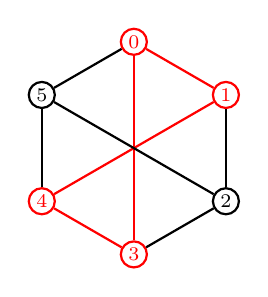
\begin{tikzpicture}[
  thick,  vertex/.style={circle,draw,inner sep=1.2pt,font=\scriptsize},  svertex/.style={circle,draw=red,text=red,inner sep=1.2pt,font=\scriptsize},  baseline=(current bounding box.north)
]
  \node[svertex] (v0) at (0.000,1.350) {0};
  \node[svertex] (v1) at (1.169,0.675) {1};
  \node[vertex] (v2) at (1.169,-0.675) {2};
  \node[svertex] (v3) at (0.000,-1.350) {3};
  \node[svertex] (v4) at (-1.169,-0.675) {4};
  \node[vertex] (v5) at (-1.169,0.675) {5};
  \draw[red] (v0) -- (v1);
  \draw[red] (v0) -- (v3);
  \draw (v0) -- (v5);
  \draw (v1) -- (v2);
  \draw[red] (v1) -- (v4);
  \draw (v2) -- (v3);
  \draw (v2) -- (v5);
  \draw[red] (v3) -- (v4);
  \draw (v4) -- (v5);
\end{tikzpicture}
\par\smallskip Graph 5
\par $L=\{\textcolor{red}{1},\textcolor{red}{3}\}$
\par $y=\left(\textcolor{red}{1},\textcolor{red}{0},\textcolor{red}{1}\right)$
\par $|E(L)\cap E(S)|=4\;\;\textcolor{red}{\boldsymbol{\times}}$
\end{minipage}\hfill\begin{minipage}[t]{0.31\textwidth}
\centering
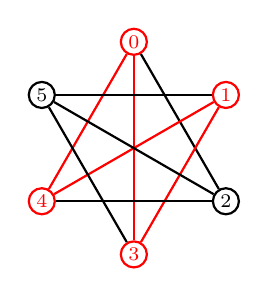
\begin{tikzpicture}[
  thick,  vertex/.style={circle,draw,inner sep=1.2pt,font=\scriptsize},  svertex/.style={circle,draw=red,text=red,inner sep=1.2pt,font=\scriptsize},  baseline=(current bounding box.north)
]
  \node[svertex] (v0) at (0.000,1.350) {0};
  \node[svertex] (v1) at (1.169,0.675) {1};
  \node[vertex] (v2) at (1.169,-0.675) {2};
  \node[svertex] (v3) at (0.000,-1.350) {3};
  \node[svertex] (v4) at (-1.169,-0.675) {4};
  \node[vertex] (v5) at (-1.169,0.675) {5};
  \draw (v0) -- (v2);
  \draw[red] (v0) -- (v3);
  \draw[red] (v0) -- (v4);
  \draw[red] (v1) -- (v3);
  \draw[red] (v1) -- (v4);
  \draw (v1) -- (v5);
  \draw (v2) -- (v4);
  \draw (v2) -- (v5);
  \draw (v3) -- (v5);
\end{tikzpicture}
\par\smallskip Graph 6
\par $L=\{\textcolor{red}{2},\textcolor{red}{3}\}$
\par $y=\left(\textcolor{red}{0},\textcolor{red}{1},\textcolor{red}{1}\right)$
\par $|E(L)\cap E(S)|=4\;\;\textcolor{red}{\boldsymbol{\times}}$
\end{minipage}
\par\medskip
\noindent
\begin{minipage}[t]{0.31\textwidth}
\centering
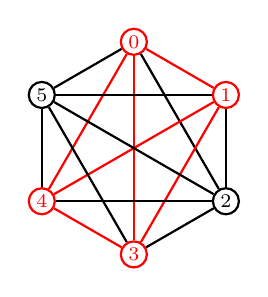
\begin{tikzpicture}[
  thick,  vertex/.style={circle,draw,inner sep=1.2pt,font=\scriptsize},  svertex/.style={circle,draw=red,text=red,inner sep=1.2pt,font=\scriptsize},  baseline=(current bounding box.north)
]
  \node[svertex] (v0) at (0.000,1.350) {0};
  \node[svertex] (v1) at (1.169,0.675) {1};
  \node[vertex] (v2) at (1.169,-0.675) {2};
  \node[svertex] (v3) at (0.000,-1.350) {3};
  \node[svertex] (v4) at (-1.169,-0.675) {4};
  \node[vertex] (v5) at (-1.169,0.675) {5};
  \draw[red] (v0) -- (v1);
  \draw (v0) -- (v2);
  \draw[red] (v0) -- (v3);
  \draw[red] (v0) -- (v4);
  \draw (v0) -- (v5);
  \draw (v1) -- (v2);
  \draw[red] (v1) -- (v3);
  \draw[red] (v1) -- (v4);
  \draw (v1) -- (v5);
  \draw (v2) -- (v3);
  \draw (v2) -- (v4);
  \draw (v2) -- (v5);
  \draw[red] (v3) -- (v4);
  \draw (v3) -- (v5);
  \draw (v4) -- (v5);
\end{tikzpicture}
\par\smallskip Graph 7
\par $L=\{\textcolor{red}{1},\textcolor{red}{2},\textcolor{red}{3}\}$
\par $y=\left(\textcolor{red}{1},\textcolor{red}{1},\textcolor{red}{1}\right)$
\par $|E(L)\cap E(S)|=6\;\;\textcolor{red}{\boldsymbol{\times}}$
\end{minipage}
\par\medskip

\noindent\textbf{Matrix Data}
\par $N=0$
\par $I=\varnothing$\quad$Y=\varnothing$
\par $Y^{+}=\varnothing$\quad$\operatorname{rank}(Y^{+})=0$
\end{document}
